\chapter{CSTR model}
\label{sec_cstr}
In this chapter we introduce the model we will use to illustrate the techniques we develop in this dissertation. The model is a simple continuously stirred tank reactor (CSTR) undergoing an exothermic, irreversible first order reaction where $A \rightarrow B$. A schematic diagram of the reactor is shown in Figure \ref{fig_cstr_diagram}. The model is taken from literature \cite{cstrmodel}.
\begin{figure}[H] 
\centering
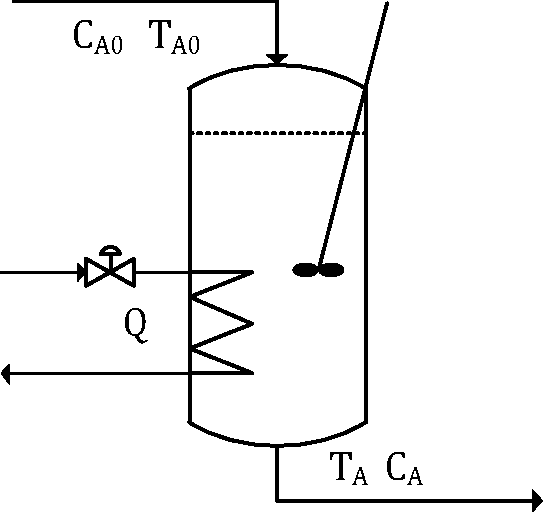
\includegraphics[scale=0.8]{cstr_diagram.pdf}
\caption{Diagram of a simple CSTR where the heat added to system is the only manipulated variable.}
\label{fig_cstr_diagram}
\end{figure}
The state space equations describing the reactor are shown in (\ref{eq_cstrmodel}) with parameters shown in Table \ref{tab_params}. The meaning of the variables is what one would expect from an intuitive understanding: $C_A$ is the concentration of species $A$, $T_R$ is the temperature of the CSTR and $Q$ is the heat added (or removed for negative $Q$) from the CSTR.
\begin{equation}
\begin{aligned}
\dot{C_A} &= f(C_A, T_R) =  \frac{F}{V}\left( C_{A0}-C_A \right) - k_0e^{\frac{-E}{RT_R}}C_A \\
\dot{T_R} &= g(C_A, T_R) = \frac{F}{V}\left(T_{A0}-T_A\right) + \frac{-\triangle H}{\rho C_p}k_0e^{\frac{-E}{RT_R}}C_A + \frac{Q}{\rho C_p V}
\end{aligned}
\label{eq_cstrmodel}
\end{equation}
\begin{table}[H]
\begin{center}
\begin{tabular}{c c c c}
\hline
$V$ & $~5.0~m^3$ & $R$ & $~8.314~\frac{kJ}{kmol.K}$ \\
$C_{A0}$ & $~1.0~\frac{kmol}{m^3}$ &$T_{A0}$ & $~310~K$ \\
$\triangle H$ & $~-4.78\times 10^{4}~\frac{kJ}{kmol}$ & $k_{0}$ & $~72\times 10^{7}~\frac{1}{min}$ \\
$E$ & $~8.314\times 10^4~\frac{kJ}{kmol}$ & $C_{p}$ & $~0.239~\frac{kJ}{kg.K}$ \\
$\rho$ & $~1000~\frac{kg}{m^3}$ & 
$F$ & $~100\times 10^{-3}~\frac{m^3}{min}$ \\
\hline
\end{tabular}
\caption{CSTR parameters}
\label{tab_params}
\end{center}
\end{table}
The CSTR model is a familiar control example. Similar models may be found in \cite{du}\cite{cervantes}\cite{pan}\cite{yazdi}. We use this model because it is low dimensional yet complex enough to illustrate the principles we investigate. CSTR models are also very popular examples to illustrate control techniques because they invariable have nonlinear dynamics and multiple steady states. Note that we have increased the volume of the reactor and reduced the rate constant from the reactor we quoted in literature. This is primarily to adjust the time scale of the transient response to be in the order of minutes and not milliseconds when moving to high temperature regions of operation.

\section{Qualitative analysis}
In this chapter we use standard mathematical tools, as found in \cite{edwardsandpenny}, to analyse the qualitative behaviour of the CSTR. By inspecting (\ref{eq_cstrmodel}) we see that the model is coupled and nonlinear. By solving (\ref{eq_cstr_statpoints}) we see that for nominal operating conditions ($Q = 0$) there exist 3 operating points (critical points) as shown in Table \ref{tab_nominalstats}.
\begin{equation}
\begin{aligned}
0 &= \frac{F}{V}\left( C_{A0}-C_A \right) - k_0e^{\frac{-E}{RT_R}}C_A \\
0 &= \frac{F}{V}\left(T_{A0}-T_A\right) + \frac{-\triangle H}{\rho C_p}k_0e^{\frac{-E}{RT_R}}C_A + \frac{Q}{\rho C_p V}
\end{aligned}
\label{eq_cstr_statpoints}
\end{equation}
\begin{table}[H]
\begin{center}
\begin{tabular}{c c c c}
\hline
Critical Point & $C_A$ & $T_R$ & Stability\\
\hline
$\left(C_A^1, T_R^1\right)$ & 0.0097 & 508.0562 & Stable Improper Node\\
$\left(C_A^2, T_R^2\right)$ & 0.4893 & 412.1302 & Unstable Saddle Point \\
$\left(C_A^3, T_R^3 \right)$ & 0.9996 & 310.0709 & Stable Improper Node \\
\hline
\end{tabular}
\caption{Nominal operating points for  the CSTR}
\label{tab_nominalstats}
\end{center}
\end{table}
The stability of the operating points were found by linearising (\ref{eq_cstrmodel}) and computing the eigenvalues of the jacobian, shown in (\ref{eq_jacobian}), at each critical point.
\begin{equation}
J(C_A, T_R) = \begin{pmatrix}
-\frac{F}{V} - k_0e^{\frac{-E}{RT_R}} & - k_0e^{\frac{-E}{RT_R}}C_A\left(\frac{E}{RT_R^2}\right) \\
\frac{-\triangle H}{\rho C_p}k_0e^{\frac{-E}{RT_R}} & -\frac{F}{V} + \frac{-\triangle H}{\rho C_p}k_0e^{\frac{-E}{RT_R}}C_A\left(\frac{E}{RT_R^2}\right) 
\end{pmatrix}
\label{eq_jacobian}
\end{equation}
In Figure \ref{fig_cstr_op_curve} we see the operating curve for the CSTR. The curve resembles the classical CSTR operating curve with all the associated potential control complexity e.g. it is possible for one set of control inputs to result in two stable operating points. This occurs due to the two stable critical points (for $Q\in (-906, 1145)$) of the system and is called input multiplicity \cite{luyben}. 

Also note that the obvious bifurcation parameter for this system is the heat input $Q$. For $Q = -906$ kJ/min we see that we no longer have three critical points but only two, and for $Q < -906$ kJ/min we only have one critical point. Likewise, for $Q = 1145$ kJ/min we see that we only have two critical points and for $Q > 1145$ kJ/min we only have one critical point. The stability of these points are shown in Table \ref{tab_bifurc}.  
\begin{figure}[H] 
\centering
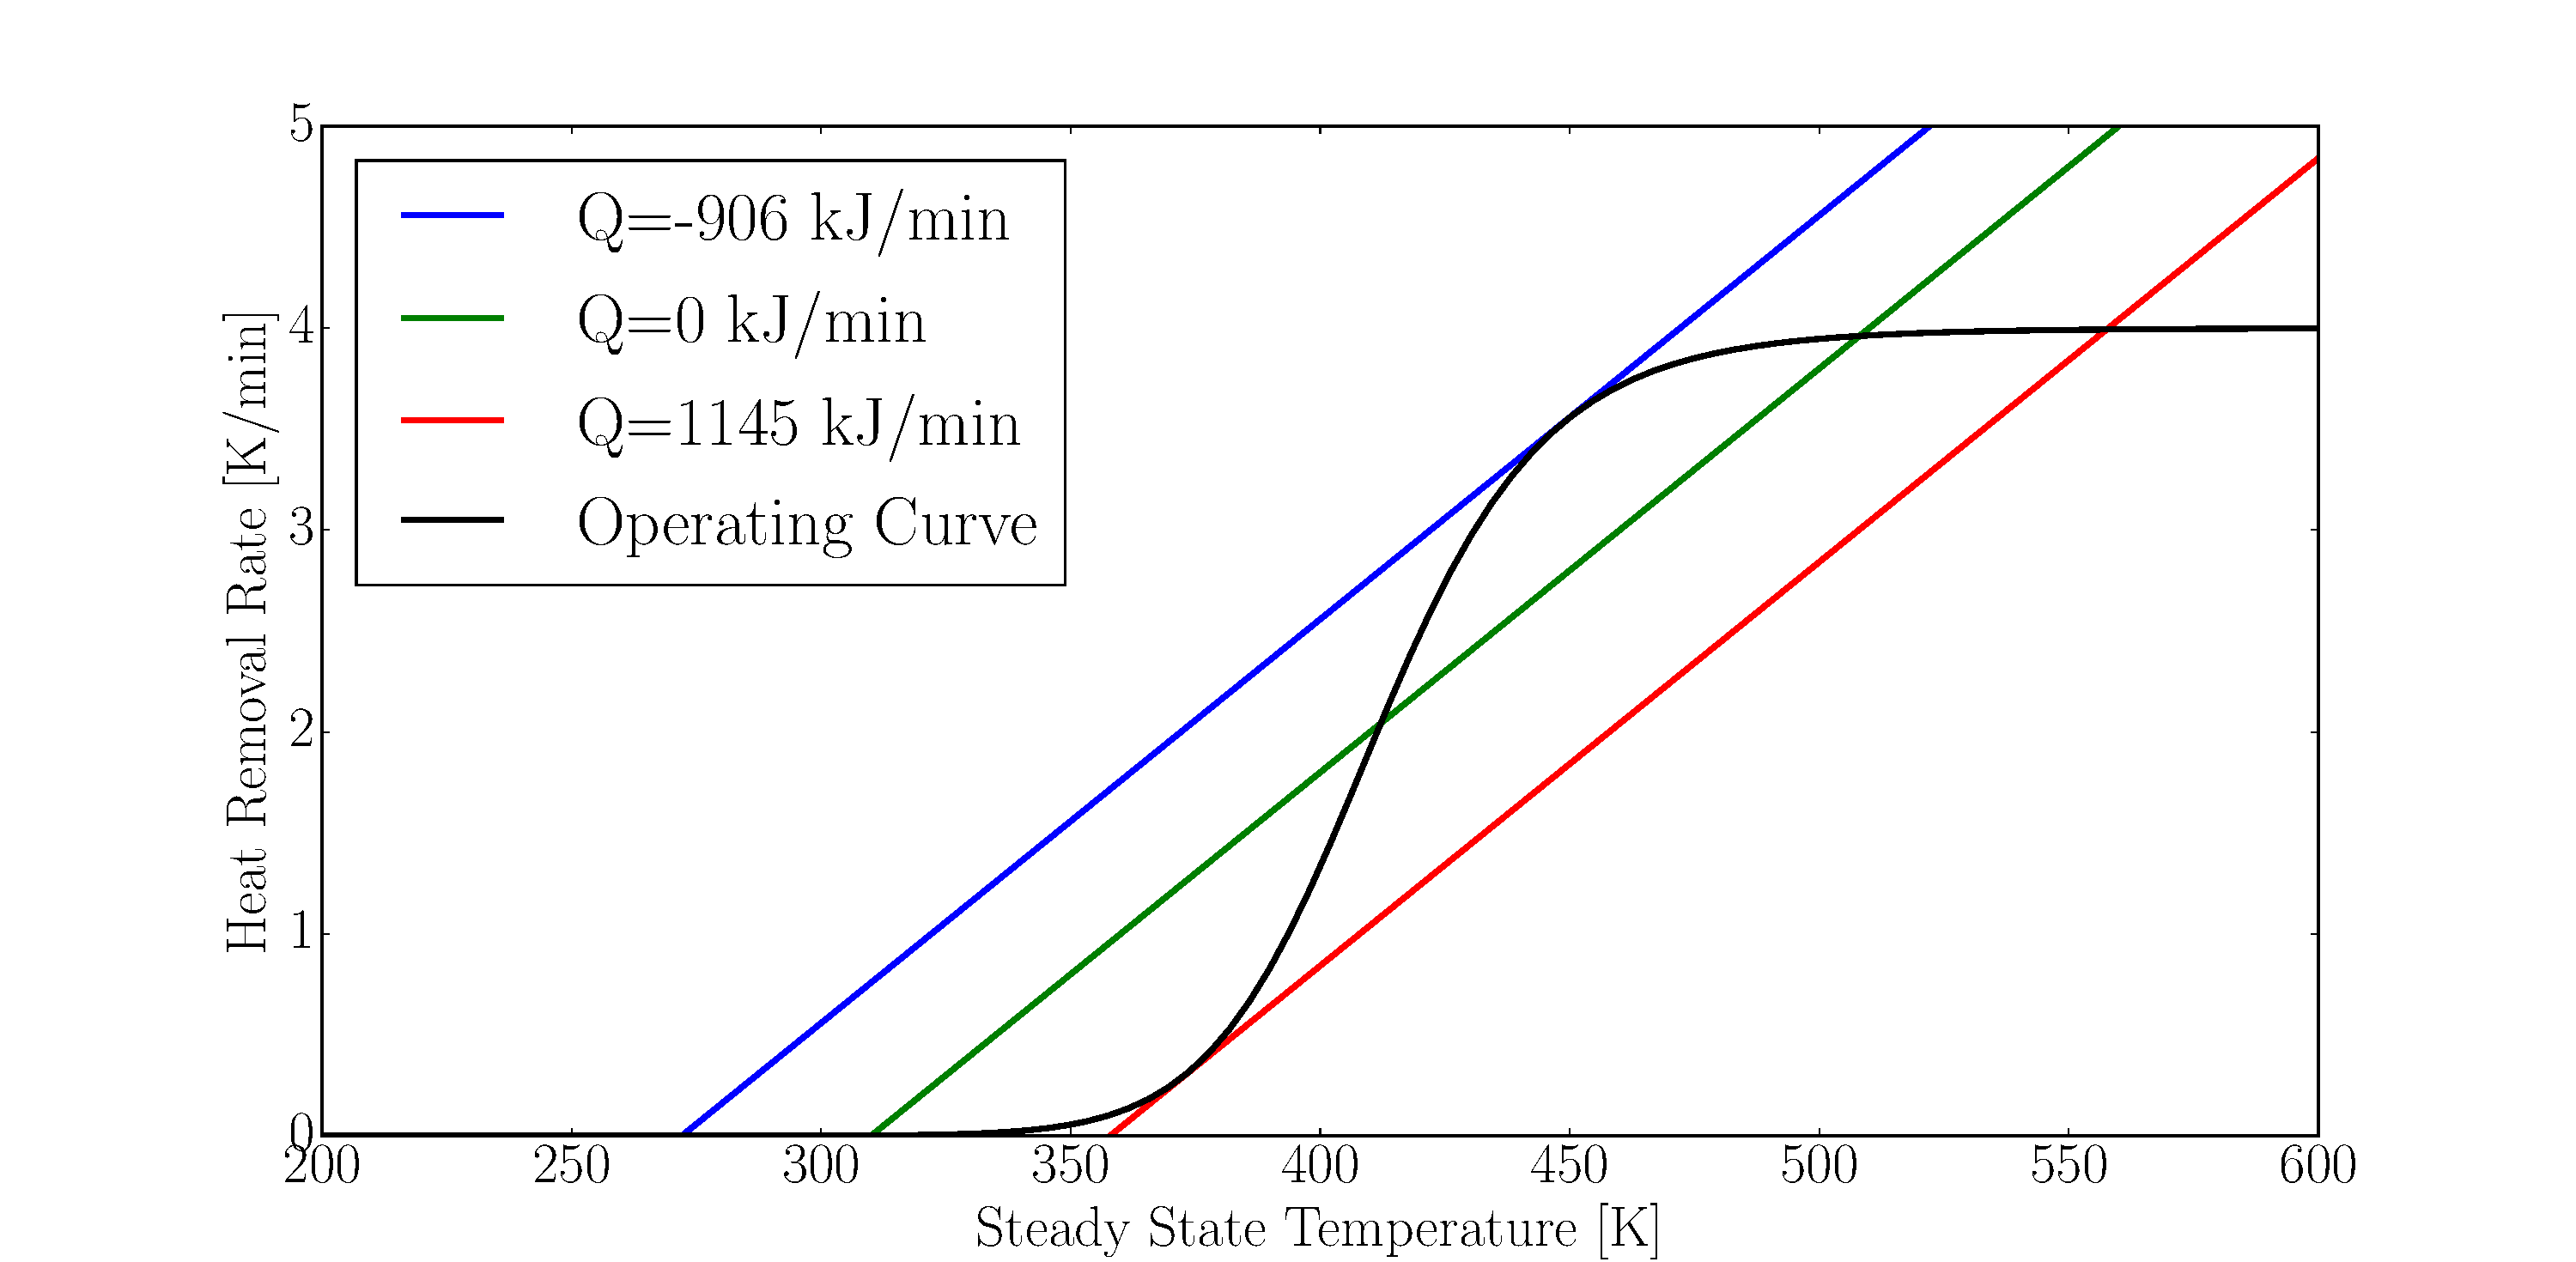
\includegraphics[width=\textwidth]{cstr_model_op_curve.pdf}
\caption{CSTR operating curve with different input curves. Nominal operating conditions are $Q=0$ kJ/min.}
\label{fig_cstr_op_curve}
\end{figure}
\begin{table}[H]
\begin{center}
\begin{tabular}{c c c c}
\hline
Heat Input & $C_A$ & $T_R$ & Stability\\
\hline
$Q = -906$ kJ/min & 0.1089 & 450.3531 & Stable Improper Node\\
$Q = -906$ kJ/min & 0.9999 & 272.1346 & Stable Improper Node \\
\hline
$Q < -906$ kJ/min & $\backsim$ & $\backsim$ & Stable Improper Node \\
\hline
$Q = 1145$ kJ/min & 0.0017 & 557.5243 & Stable Improper Node\\
$Q = 1145$ kJ/min & 0.9263 & 372.5959 & Stable Improper Node \\
\hline
$Q > 1145$ kJ/min & $\backsim$ & $\backsim$ & Stable Improper Node \\
\hline
\end{tabular}
\caption{Bifurcation analysis of the CSTR at different heat input values. The $\backsim$ notation indicates that the operating point depends on the precise value of $Q$.}
\label{tab_bifurc}
\end{center}
\end{table}
The multiple stable critical points for $Q\in [-906, 1145]$ kJ/min make control of this system challenging. For example consider a situation where one starts at some point on the black line but below the green line in Figure \ref{fig_cstr_op_curve}. If one wishes to move to the high temperature low concentration stable operating point large, non-smooth, controller action will be required. By slowly heating up the CSTR the green line will gradually move to the right and this will push the system, somewhat counter-intuitively, towards the low temperature high concentration critical point. The instability of the middle operating point causes this behaviour. It is necessary to quickly heat up the CSTR so that the green line jumps below the current operating point on the black line. The self-regulatory nature of the CSTR will then move the system to the desired operating point.   

\section{Nonlinear model}
In this chapter we evaluate the transient response of the CSTR. The nonlinear differential equation shown in (\ref{eq_cstrmodel}) is intractably difficult to solve analytically. For this reason we will use a numerical method, specifically the Runge-Kutta method \cite{edwardsandpenny}, to simulate the transient response. We chose the Runge-Kutta method because it is an explicit, fourth order accurate method which is easy to implement.

For completeness we show the method here. Suppose we have an autonomous ordinary differential equation as shown in (\ref{eq_ode}) and we require its solution over $[t_a, t_b]$. This is an initial value problem; for the sake of brevity we assume that a unique solution always exists.
\begin{equation}
\begin{aligned}
&\dot{x}(t) = f(x(t)) \\
&\text{with } x(t) = x_a \text{ for } t=t_a
\end{aligned}
\label{eq_ode}
\end{equation}
Furthermore, suppose we discretise the time domain such that $[t_a, t_b] = [t_0=t_a, t_1= t_a+ h, t_2=t_a+ 2h,...,t_T = t_b]$. Then the scheme shown in (\ref{eq_rk}) is called the Runge-Kutta method. For sufficiently small time steps, $h$, the method is stable and convergent.
\begin{equation}
\begin{aligned}
x_{t+1} &= x_{t} + \frac{h}{6}\left(k_1 + 2k_2 + 2k_3 +k4\right) \\
k_1 &= f(x_t) \\
k_2 &= f(x_t + \frac{h}{2}k_1) \\
k_3 &= f(x_t+ \frac{h}{2}k_2) \\
k_4 &= f(x_t+ hk_3) \\
\end{aligned}
\label{eq_rk}
\end{equation}  
By applying the Runge-Kutta method to the CSTR we have Figures \ref{fig_cstr_nl_1} and \ref{fig_cstr_nl_2}. It is clear that the dynamics are faster (almost two orders of magnitude) when moving to the higher temperature operating point than they are when moving to the lower temperature operating point. The impact of the nonlinear kinetics is seen here. 
\begin{figure}[H] 
\centering
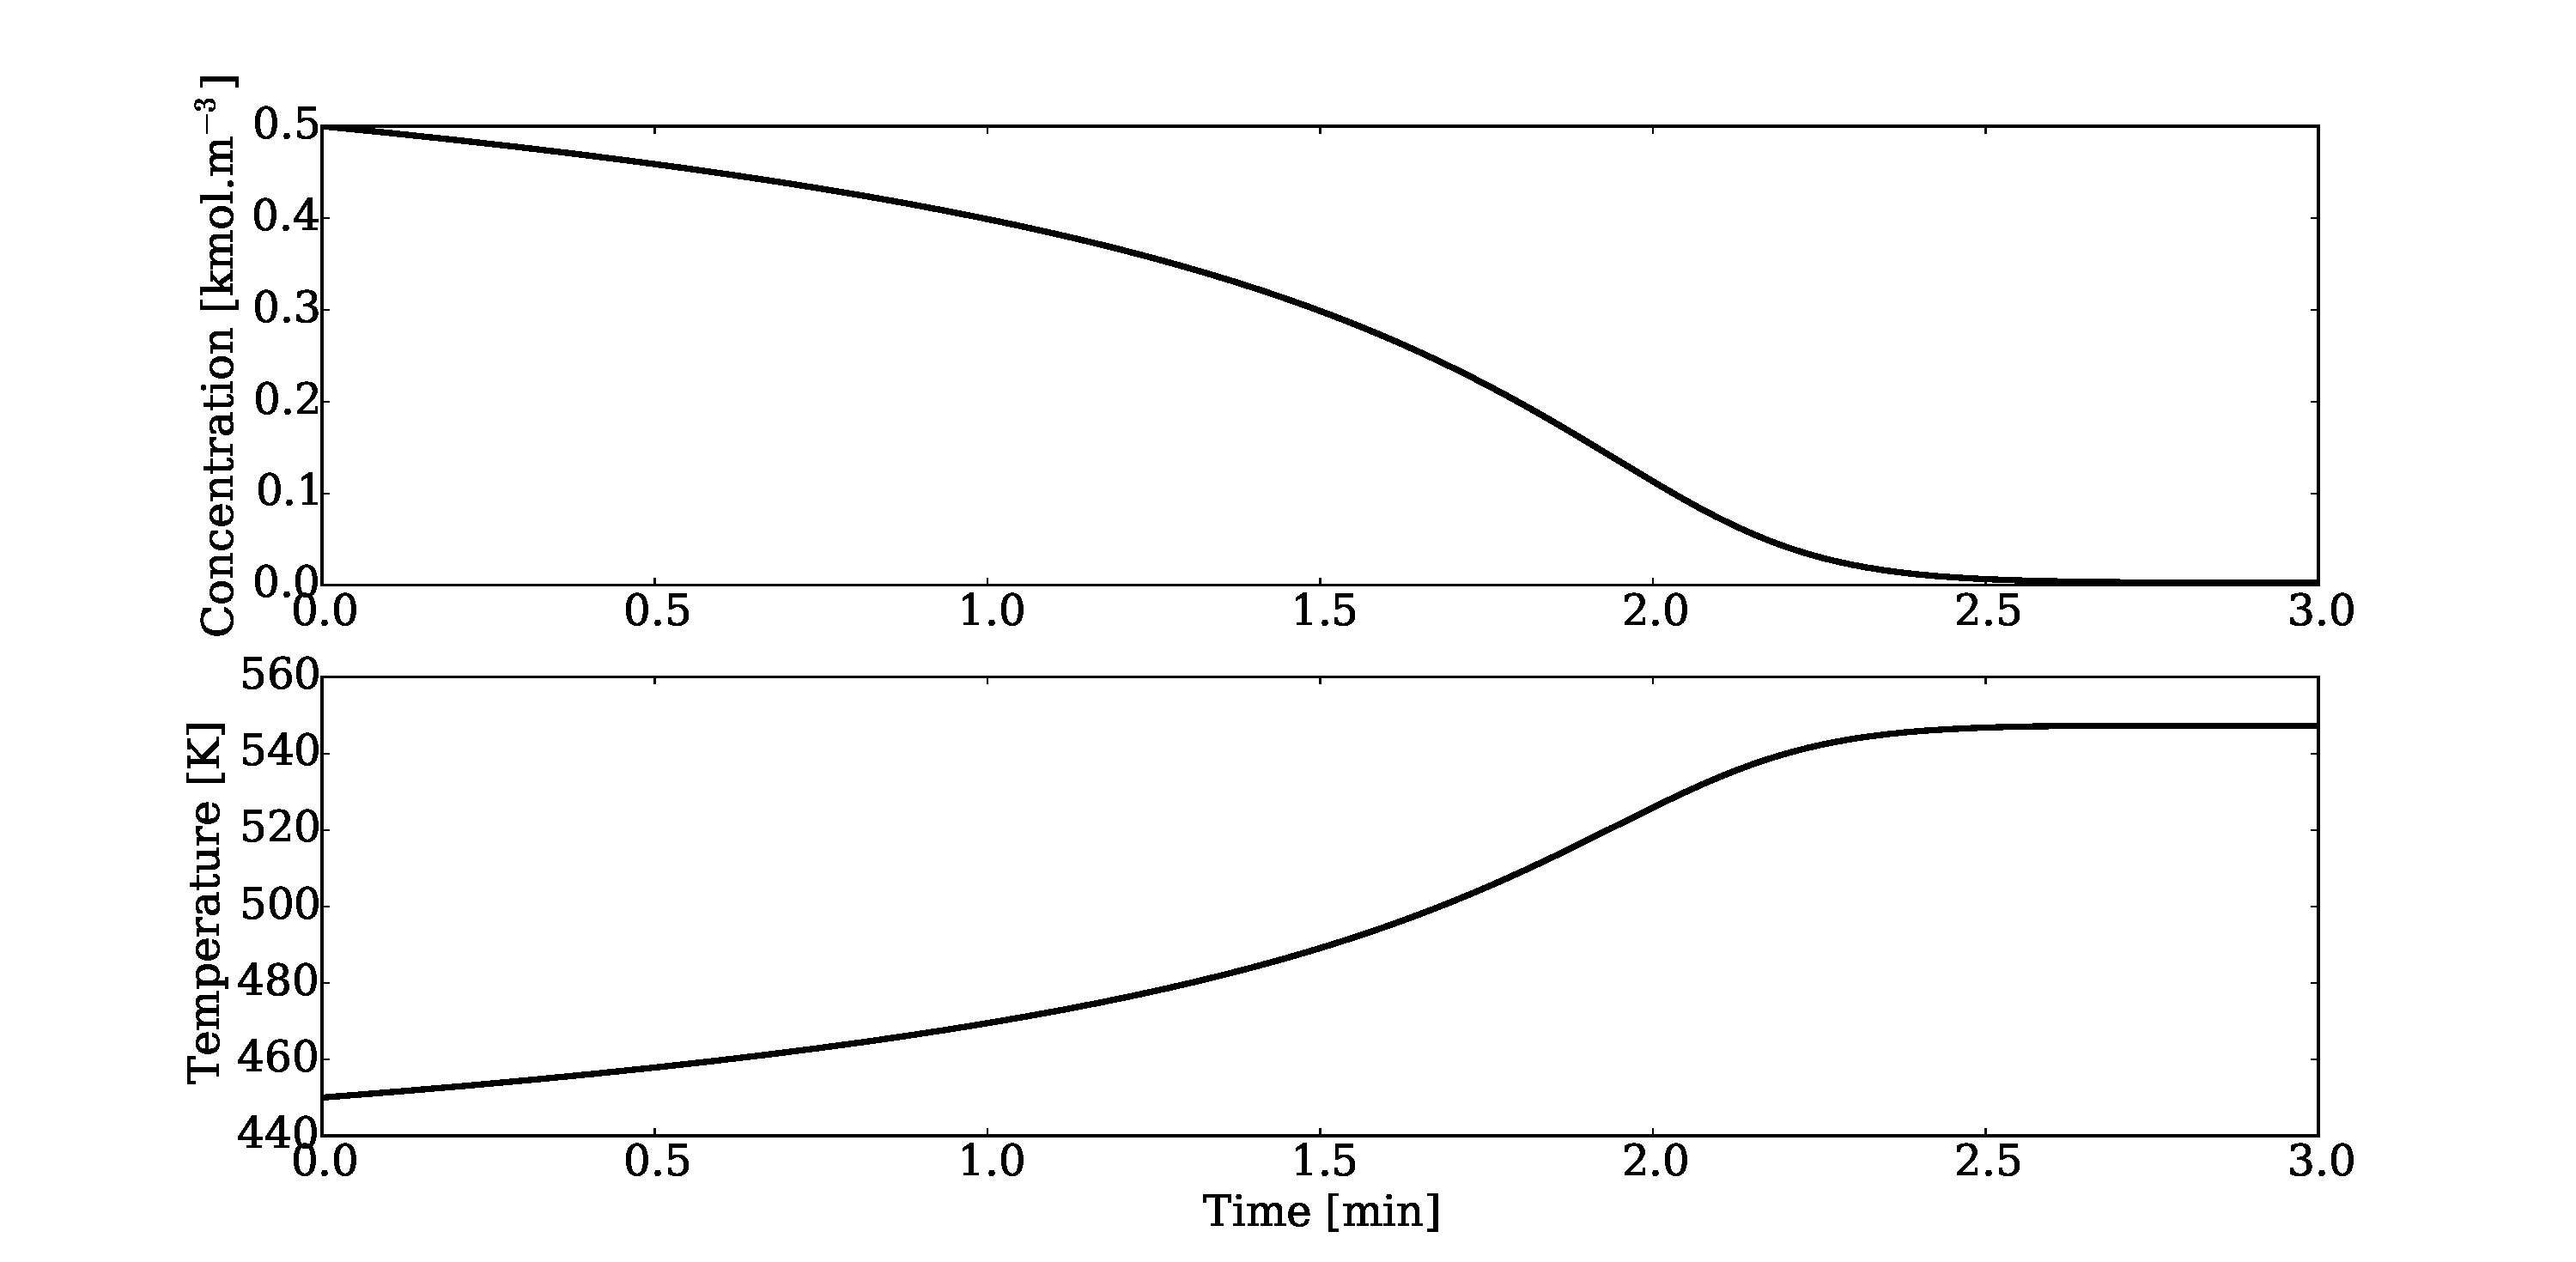
\includegraphics[width=\textwidth]{cstr_nl_1.pdf}
\caption{Transient response of the CSTR under nominal operating conditions with initial condition $(0.5, 450)$ and $h=0.1$.}
\label{fig_cstr_nl_1}
\end{figure}
\begin{figure}[H] 
\centering
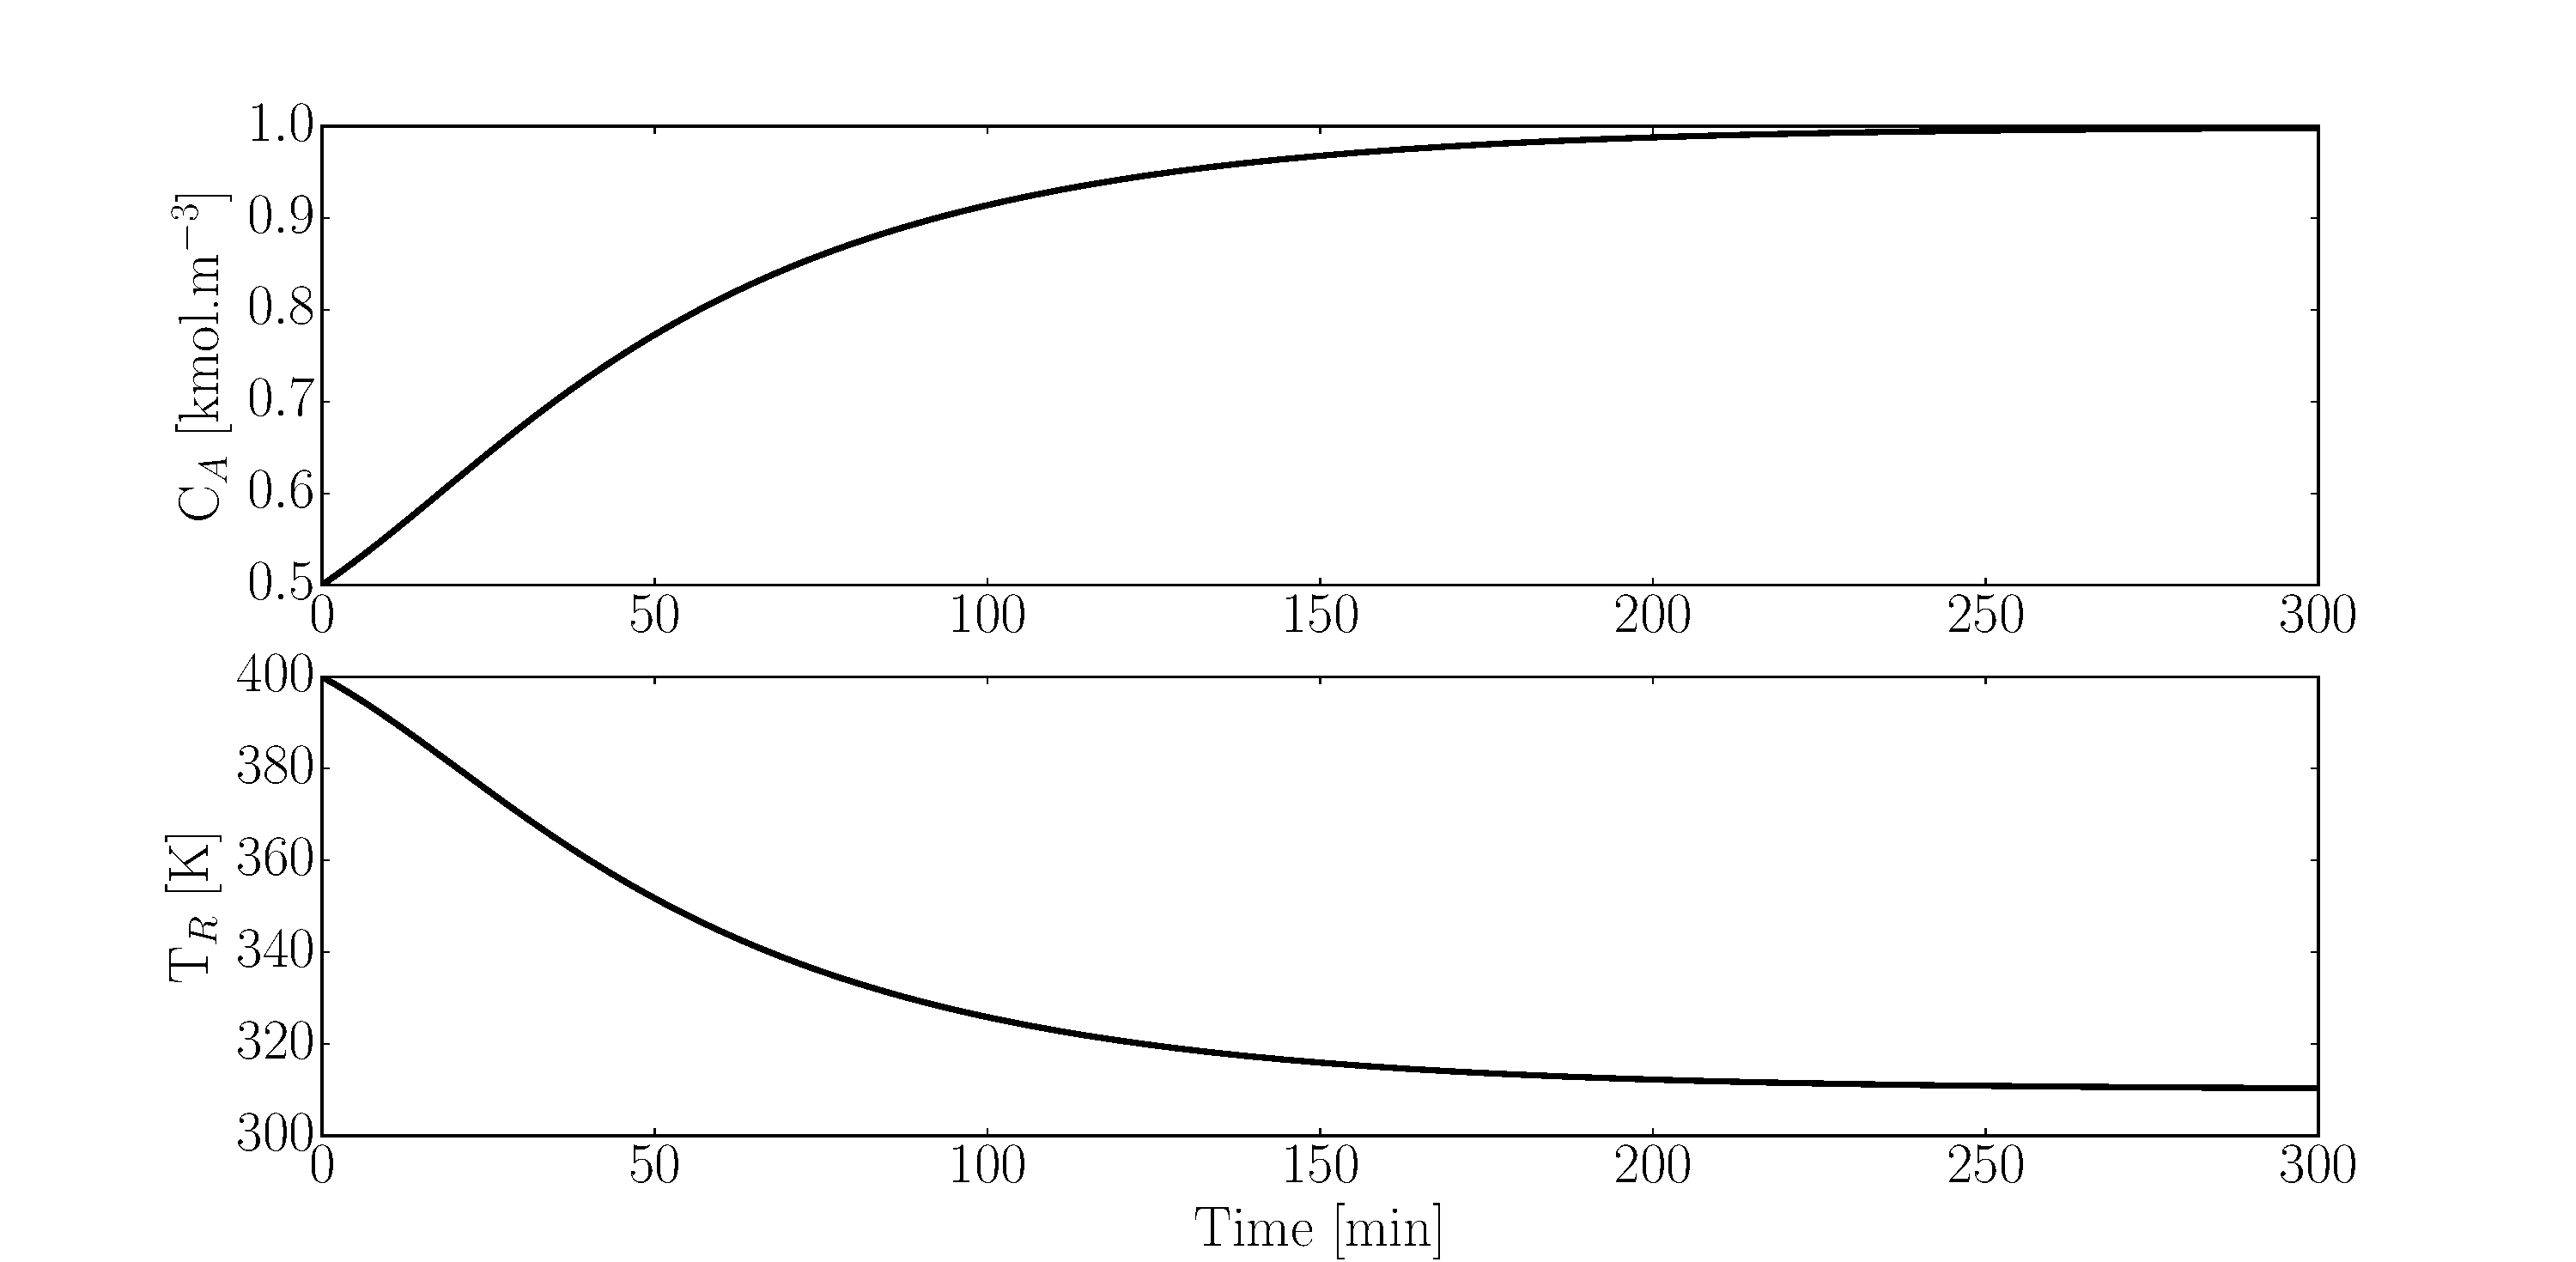
\includegraphics[width=\textwidth]{cstr_nl_2.pdf}
\caption{Transient response of the CSTR under nominal operating conditions with initial condition $(0.5, 400)$ and $h=0.1$.}
\label{fig_cstr_nl_2}
\end{figure}
It is often desirable to linearise a nonlinear system about some point, usually the operating point, to simplify the model. Computationally this is advantageous because linear techniques (e.g. linear optimisation) is usually significantly faster than nonlinear techniques. Practically linearisation is only valid in a small region around the point of linearisation. If the system moves away from the linearisation point the linear approximation can become grossly inaccurate. 

Based on Figure \ref{fig_cstr_nl_1}, where the dynamics are fast, we can venture a guess that linearisation will be a bad approximation, except for a very small time period, of plant behaviour because the states will rapidly move away from the point of linearisation.

On the other hand, based on Figure \ref{fig_cstr_nl_2}, we can venture a guess that linearisation will be a fair approximation of plant behaviour for a meaningful period of time because the dynamics are slow.

\section{Linearised models}
Linear approximations used for modelling and control are very common both in practice and literature \cite{luyben}. Furthermore, the approach of using multiple piecewise affine (linear) functions for control, based on linearisation around critical points, has also been investigated in literature \cite{du}\cite{kvasnica}. Typically the state domain is discretised into regimes and the linear approximation of the model in each regime is used for control. We will also use linear models for the purposes of control.  It is therefore prudent to investigate linearisation techniques.

First we present a linearisation technique. Consider an arbitrary point in the state space $(C_A^*, T_R^*)$. Then (\ref{eq_lin}) is the general linearised model around $(C_A^*, T_R^*)$ using the notation of (\ref{eq_cstrmodel}).
\begin{equation}
\begin{pmatrix}
\dot{C_A} \\ \dot{T_R}
\end{pmatrix} = \begin{pmatrix}
f(C_A^*, T_R^*) \\ g(C_A^*, T_R^*)
\end{pmatrix} + J(C_A^*, T_R^*) \left( \begin{pmatrix}
C_A \\ T_R
\end{pmatrix} - \begin{pmatrix}
C_A^* \\ T_R^* 
\end{pmatrix}\right)
\label{eq_lin}
\end{equation}
It is often desirable to change the variables such that (\ref{eq_lin}) has no constant terms. This change of variables, which holds even if the linearisation point is not a critical point of the model, is shown in (\ref{eq_change_vars}). 
\begin{equation}
\begin{pmatrix}
\tilde{C}_A \\ \tilde{T}_R
\end{pmatrix} = \begin{pmatrix}
C_A \\ T_R
\end{pmatrix} - J(C_A^*, T_R^*)^{-1}\left(J(C_A^*, T_R^*)\begin{pmatrix}
C_A^* \\ T_R^* 
\end{pmatrix} - \begin{pmatrix}
f(C_A^*, T_R^*) \\ g(C_A^*, T_R^*)
\end{pmatrix}_{Q=0} \right)
\label{eq_change_vars}
\end{equation}
We then have (\ref{eq_lin2}). Note that the input term $B$ originates from $\begin{pmatrix}
f(C_A^*, T_R^*) \\ g(C_A^*, T_R^*)
\end{pmatrix}$ and in (\ref{eq_change_vars}) we specifically set it to zero so that it is not removed.
\begin{equation}
\frac{d}{dx}\begin{pmatrix}
\tilde{C_A} \\ \tilde{T_R}
\end{pmatrix} =  J(C_A^*, T_R^*)\begin{pmatrix}
\tilde{C}_A \\ \tilde{T}_R
\end{pmatrix} + B(C_A^*, T_R^*)Q
\label{eq_lin2}
\end{equation}
We now use the bilinear transform (also known as Tustin's transform) to convert (\ref{eq_lin2}) into the discrete equation (\ref{eq_rkss}). Note that (\ref{eq_rkss}) implicitly depends on the sampling time.
\begin{equation}
\begin{pmatrix}
\tilde{C}_A \\ \tilde{T}_R
\end{pmatrix}_{t+1} = A(C_A^*, T_R^*) \begin{pmatrix}
\tilde{C}_A \\ \tilde{T}_R
\end{pmatrix}_{t} + B(C_A^*, T_R^*)Q 
\label{eq_rkss}
\end{equation}
Note that $Q$ is the heat input to the system. Note that we need to add back the offset we removed in the change of variables step (\ref{eq_change_vars}) when we want to physically interpret the results of applying (\ref{eq_rkss}).

Next we briefly investigate the accuracy of the linear models. In all the subsequent figures the first subplot illustrates the accuracy of the linear model if the initial value is close to the point of linearisation and the second subplot illustrates the accuracy when the initial value is further away from the point of linearisation.

Figure \ref{fig_cstr_lin_1} shows the state space response of the linear model which was linearised around the high temperature, low concentration stable operating point $(C_A^1,T_R^1)$ as defined in Table \ref{tab_nominalstats}.
\begin{figure}[H] 
\centering
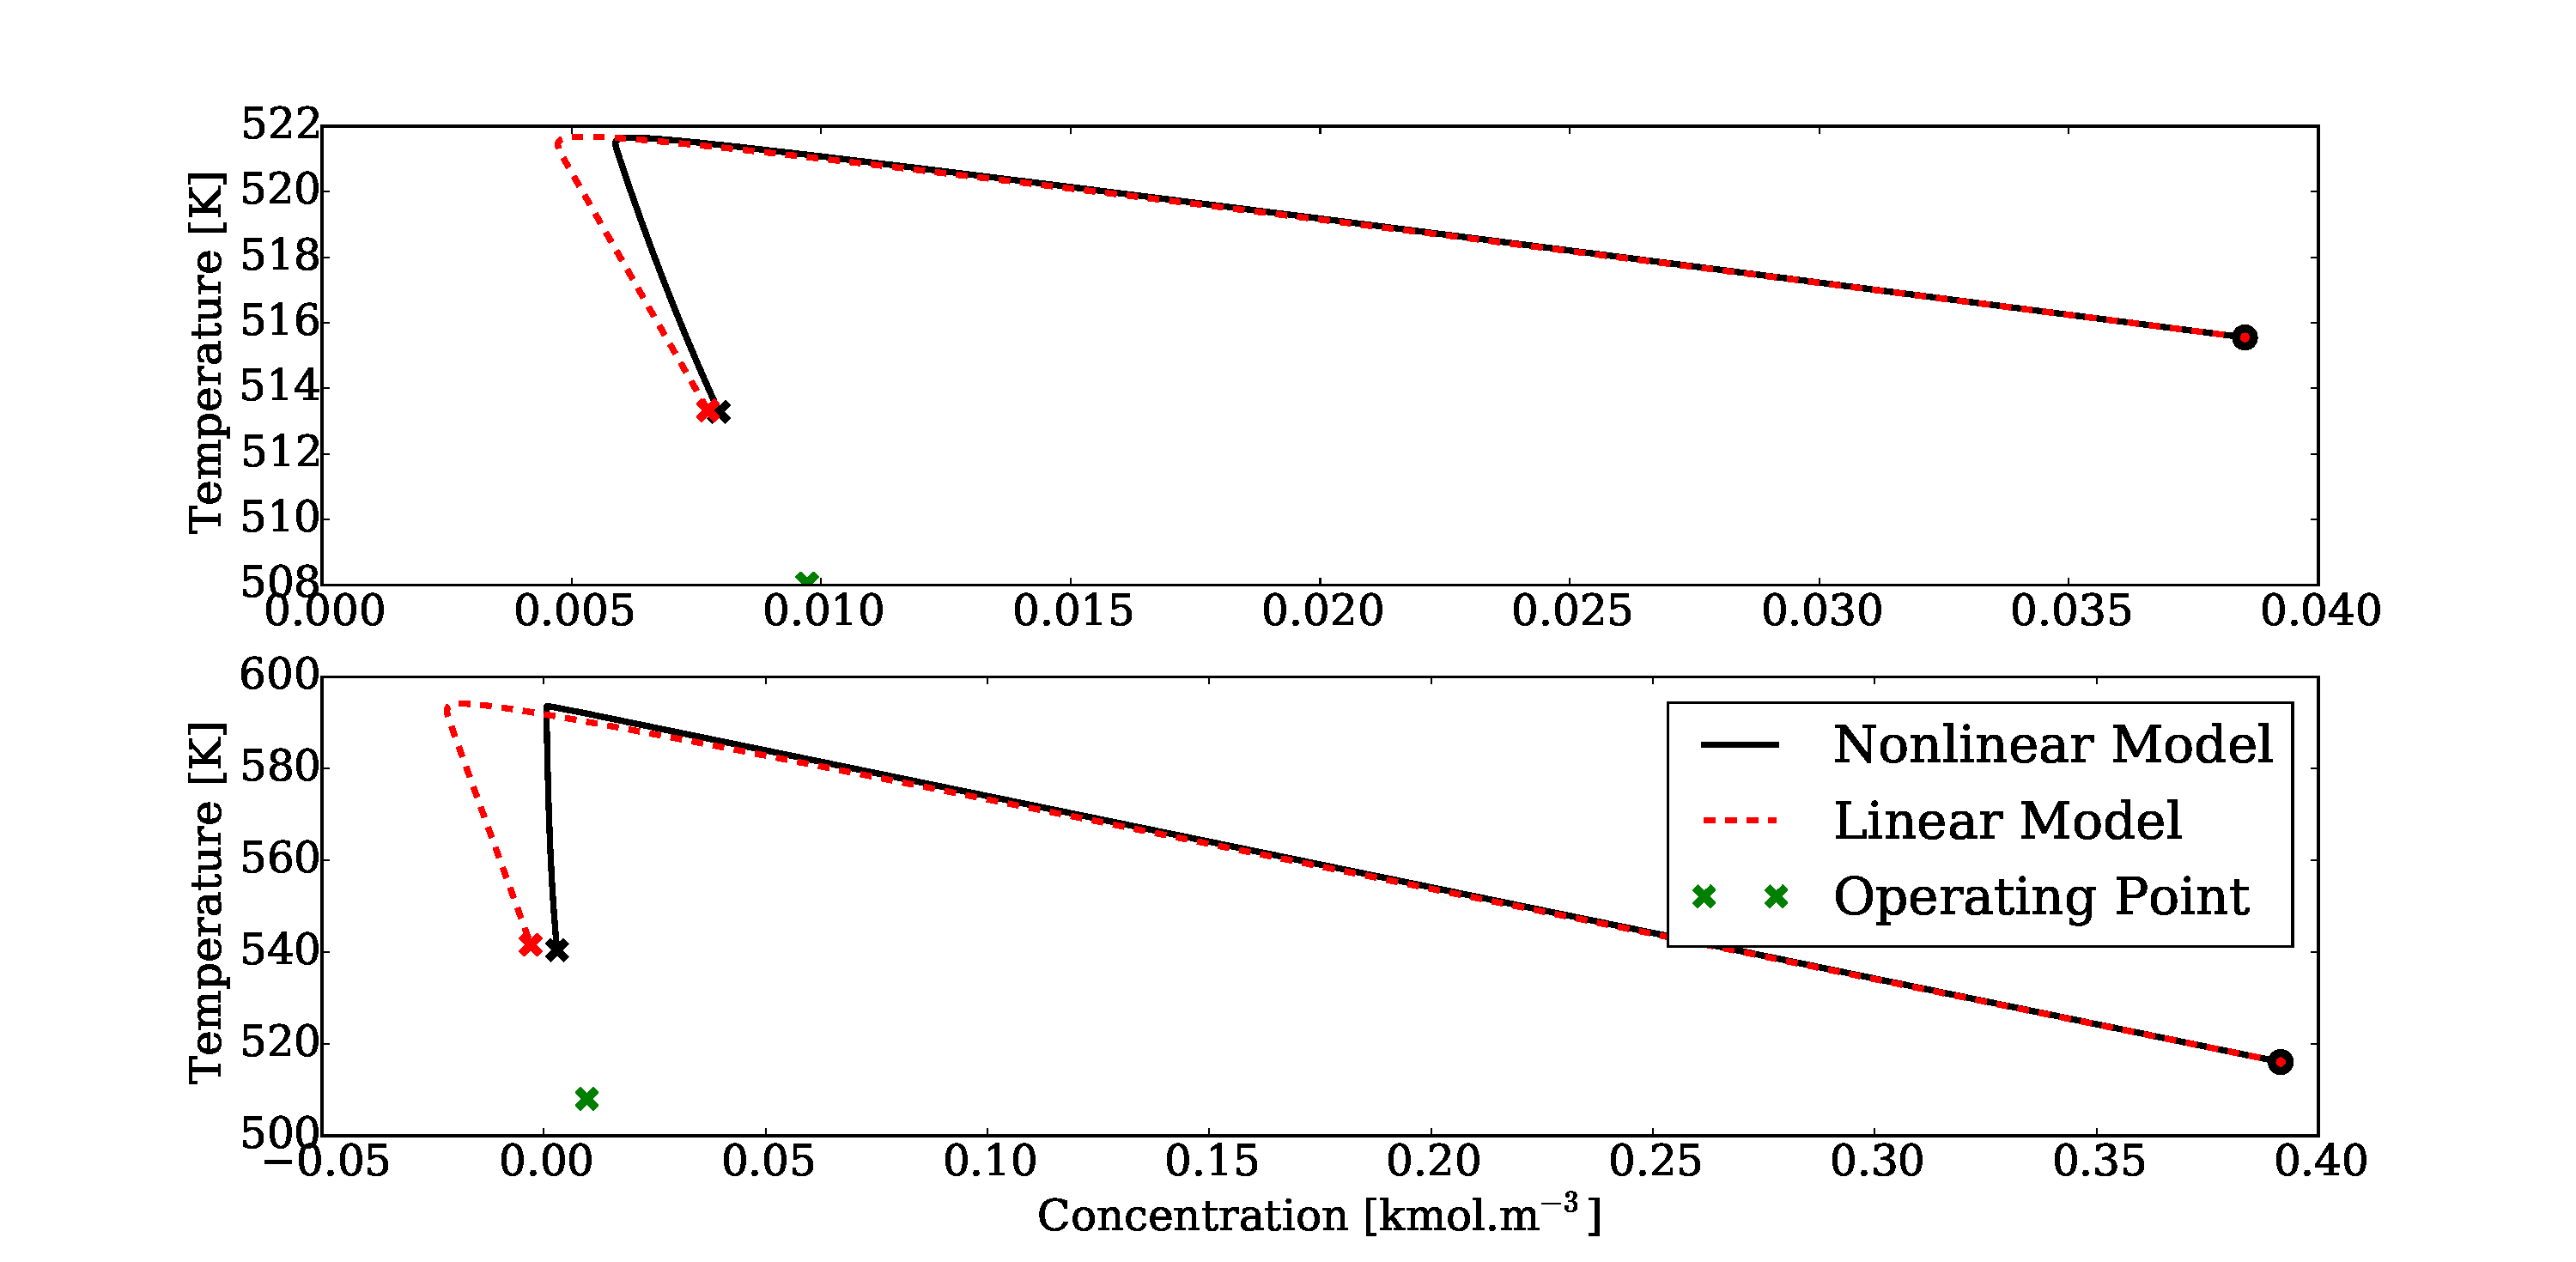
\includegraphics[width=\textwidth]{cstr_lin_1.pdf}
\caption{State space response of the CSTR under nominal operating conditions linearised around $(C_A^1,T_R^1)$ with different initial conditions. The dot indicates where the simulation started and the cross where it finished.}
\label{fig_cstr_lin_1}
\end{figure}
We see that the linear approximation is quite accurate if the initial condition is close to the linearisation point (as expected). If the initial condition is further away the approximation is less accurate.

In Figure \ref{fig_cstr_lin_2} we see the state space response of the CSTR using the linear model linearised around the unstable operating point. Clearly this approximation is less accurate because the system tend to move away from operating point rather than towards it. 
\begin{figure}[H] 
\centering
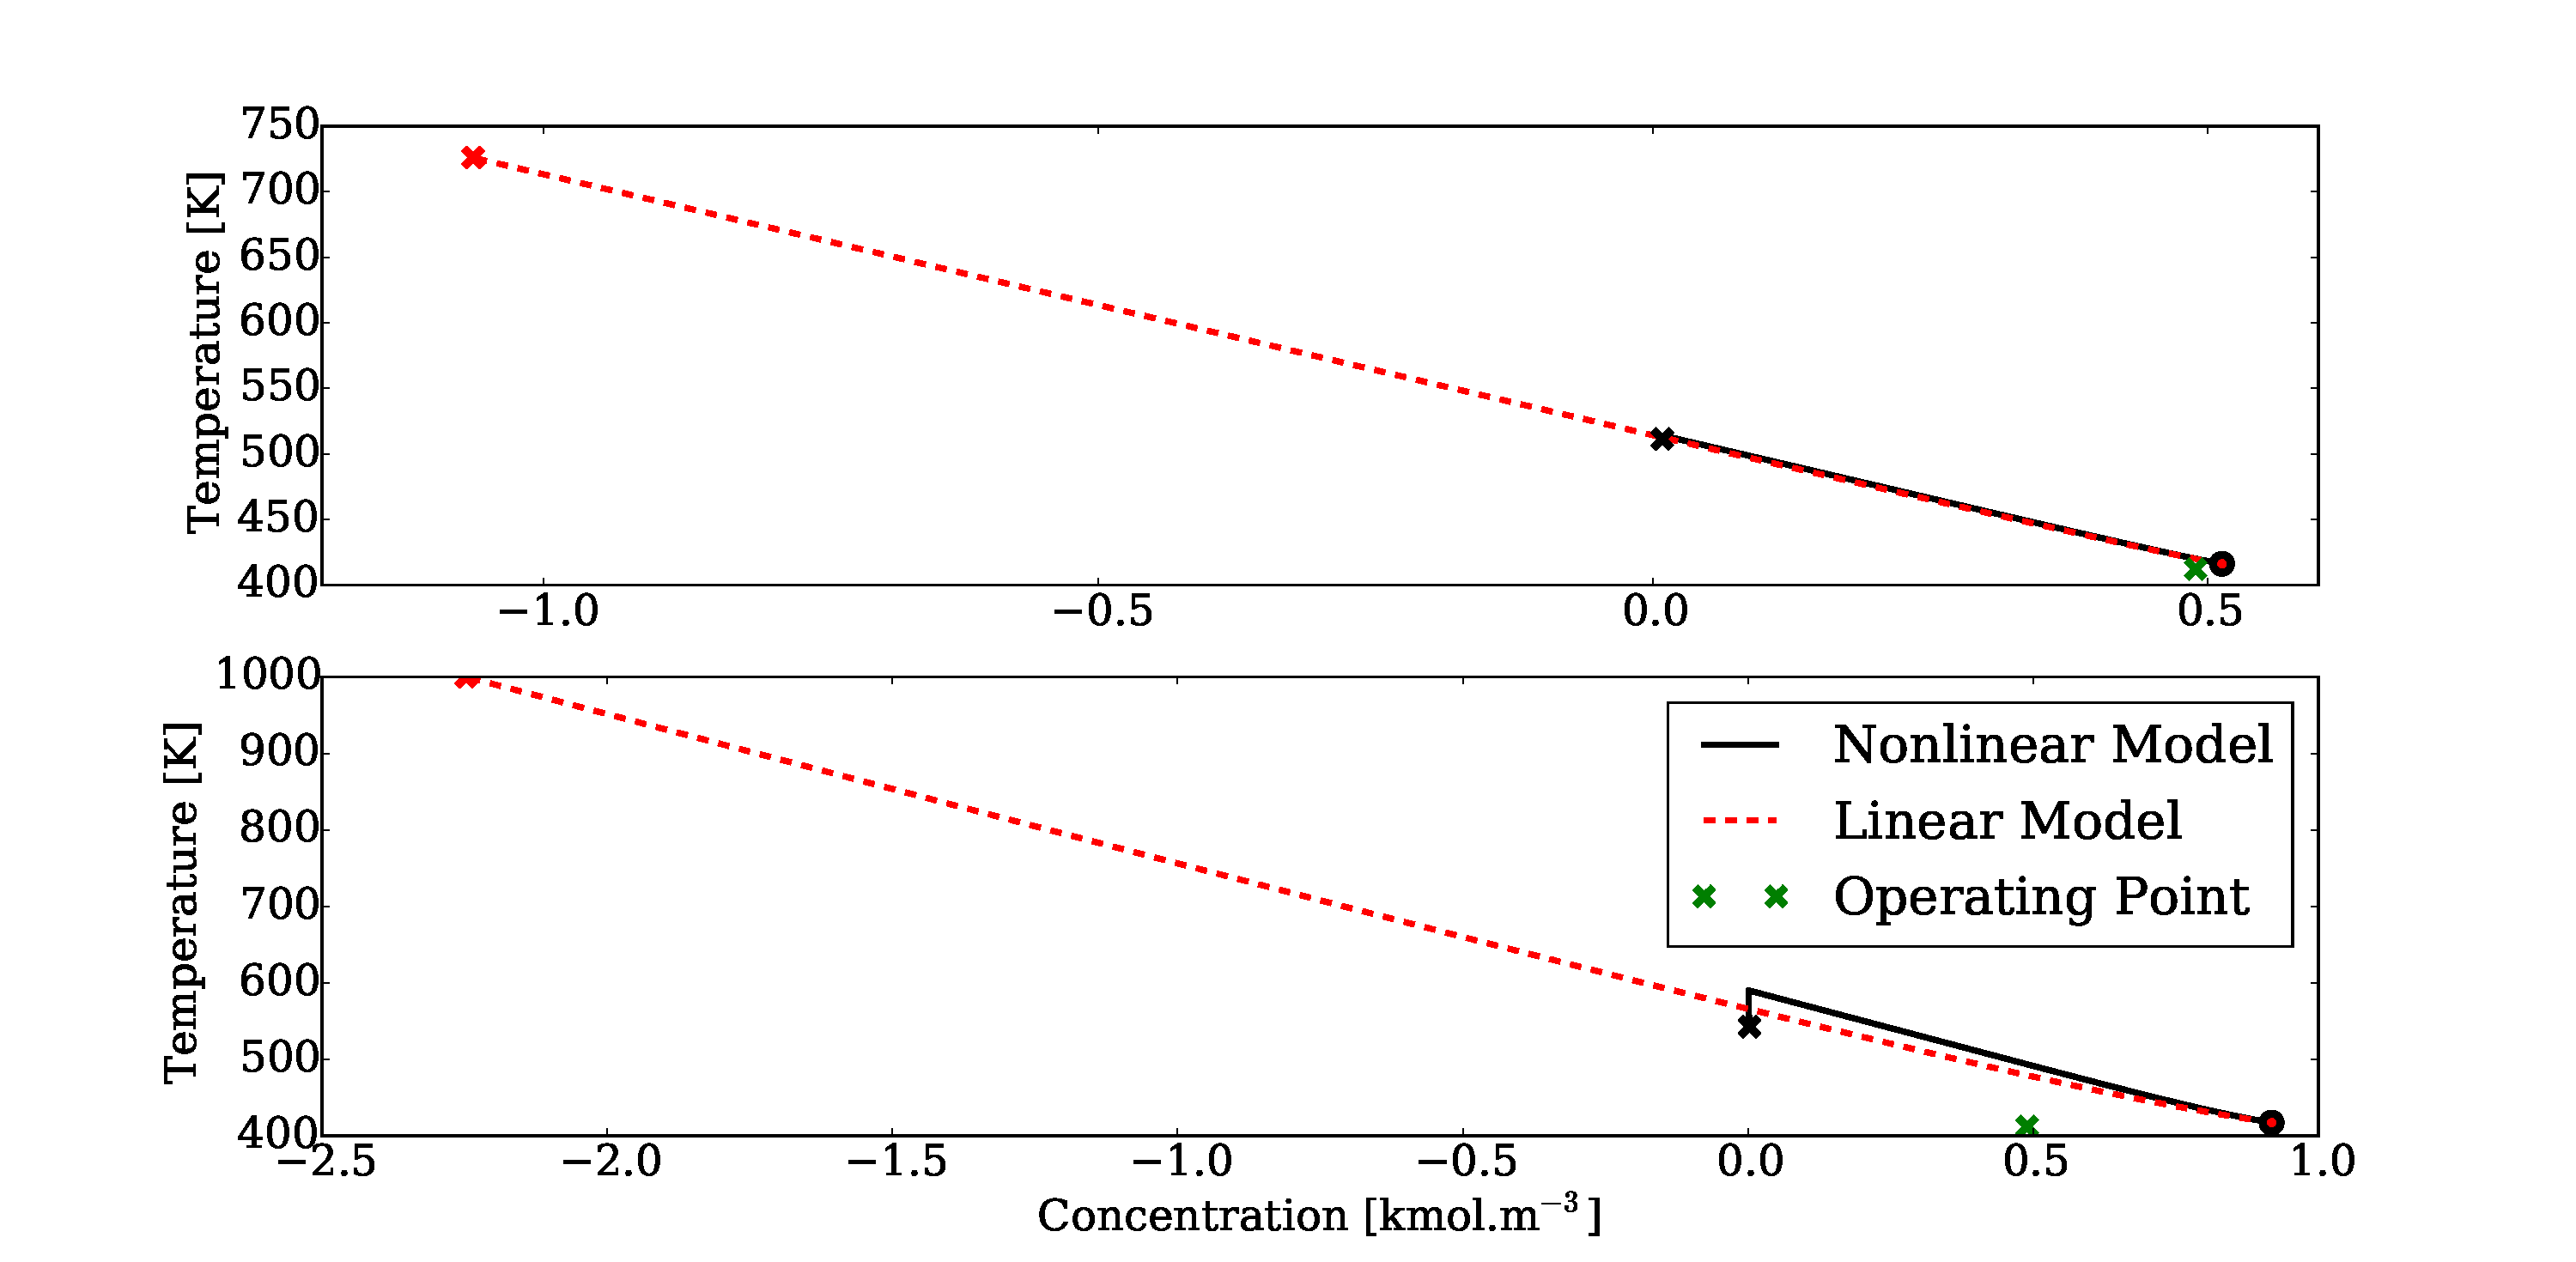
\includegraphics[width=\textwidth]{cstr_lin_2.pdf}
\caption{State space response of the CSTR under nominal operating conditions linearised around $(C_A^2,T_R^2)$ with different initial conditions. The dot indicates where the simulation started and the cross where it finished.}
\label{fig_cstr_lin_2}
\end{figure}
If we want to use the linear model around the unstable operating point we will need to effect control to keep it within some region where the model is accurate.

In Figure \ref{fig_cstr_lin_3} we have the state space response of the CSTR under nominal conditions, like before, except that we have now linearised around the low temperature high concentration operating point. 
\begin{figure}[H] 
\centering
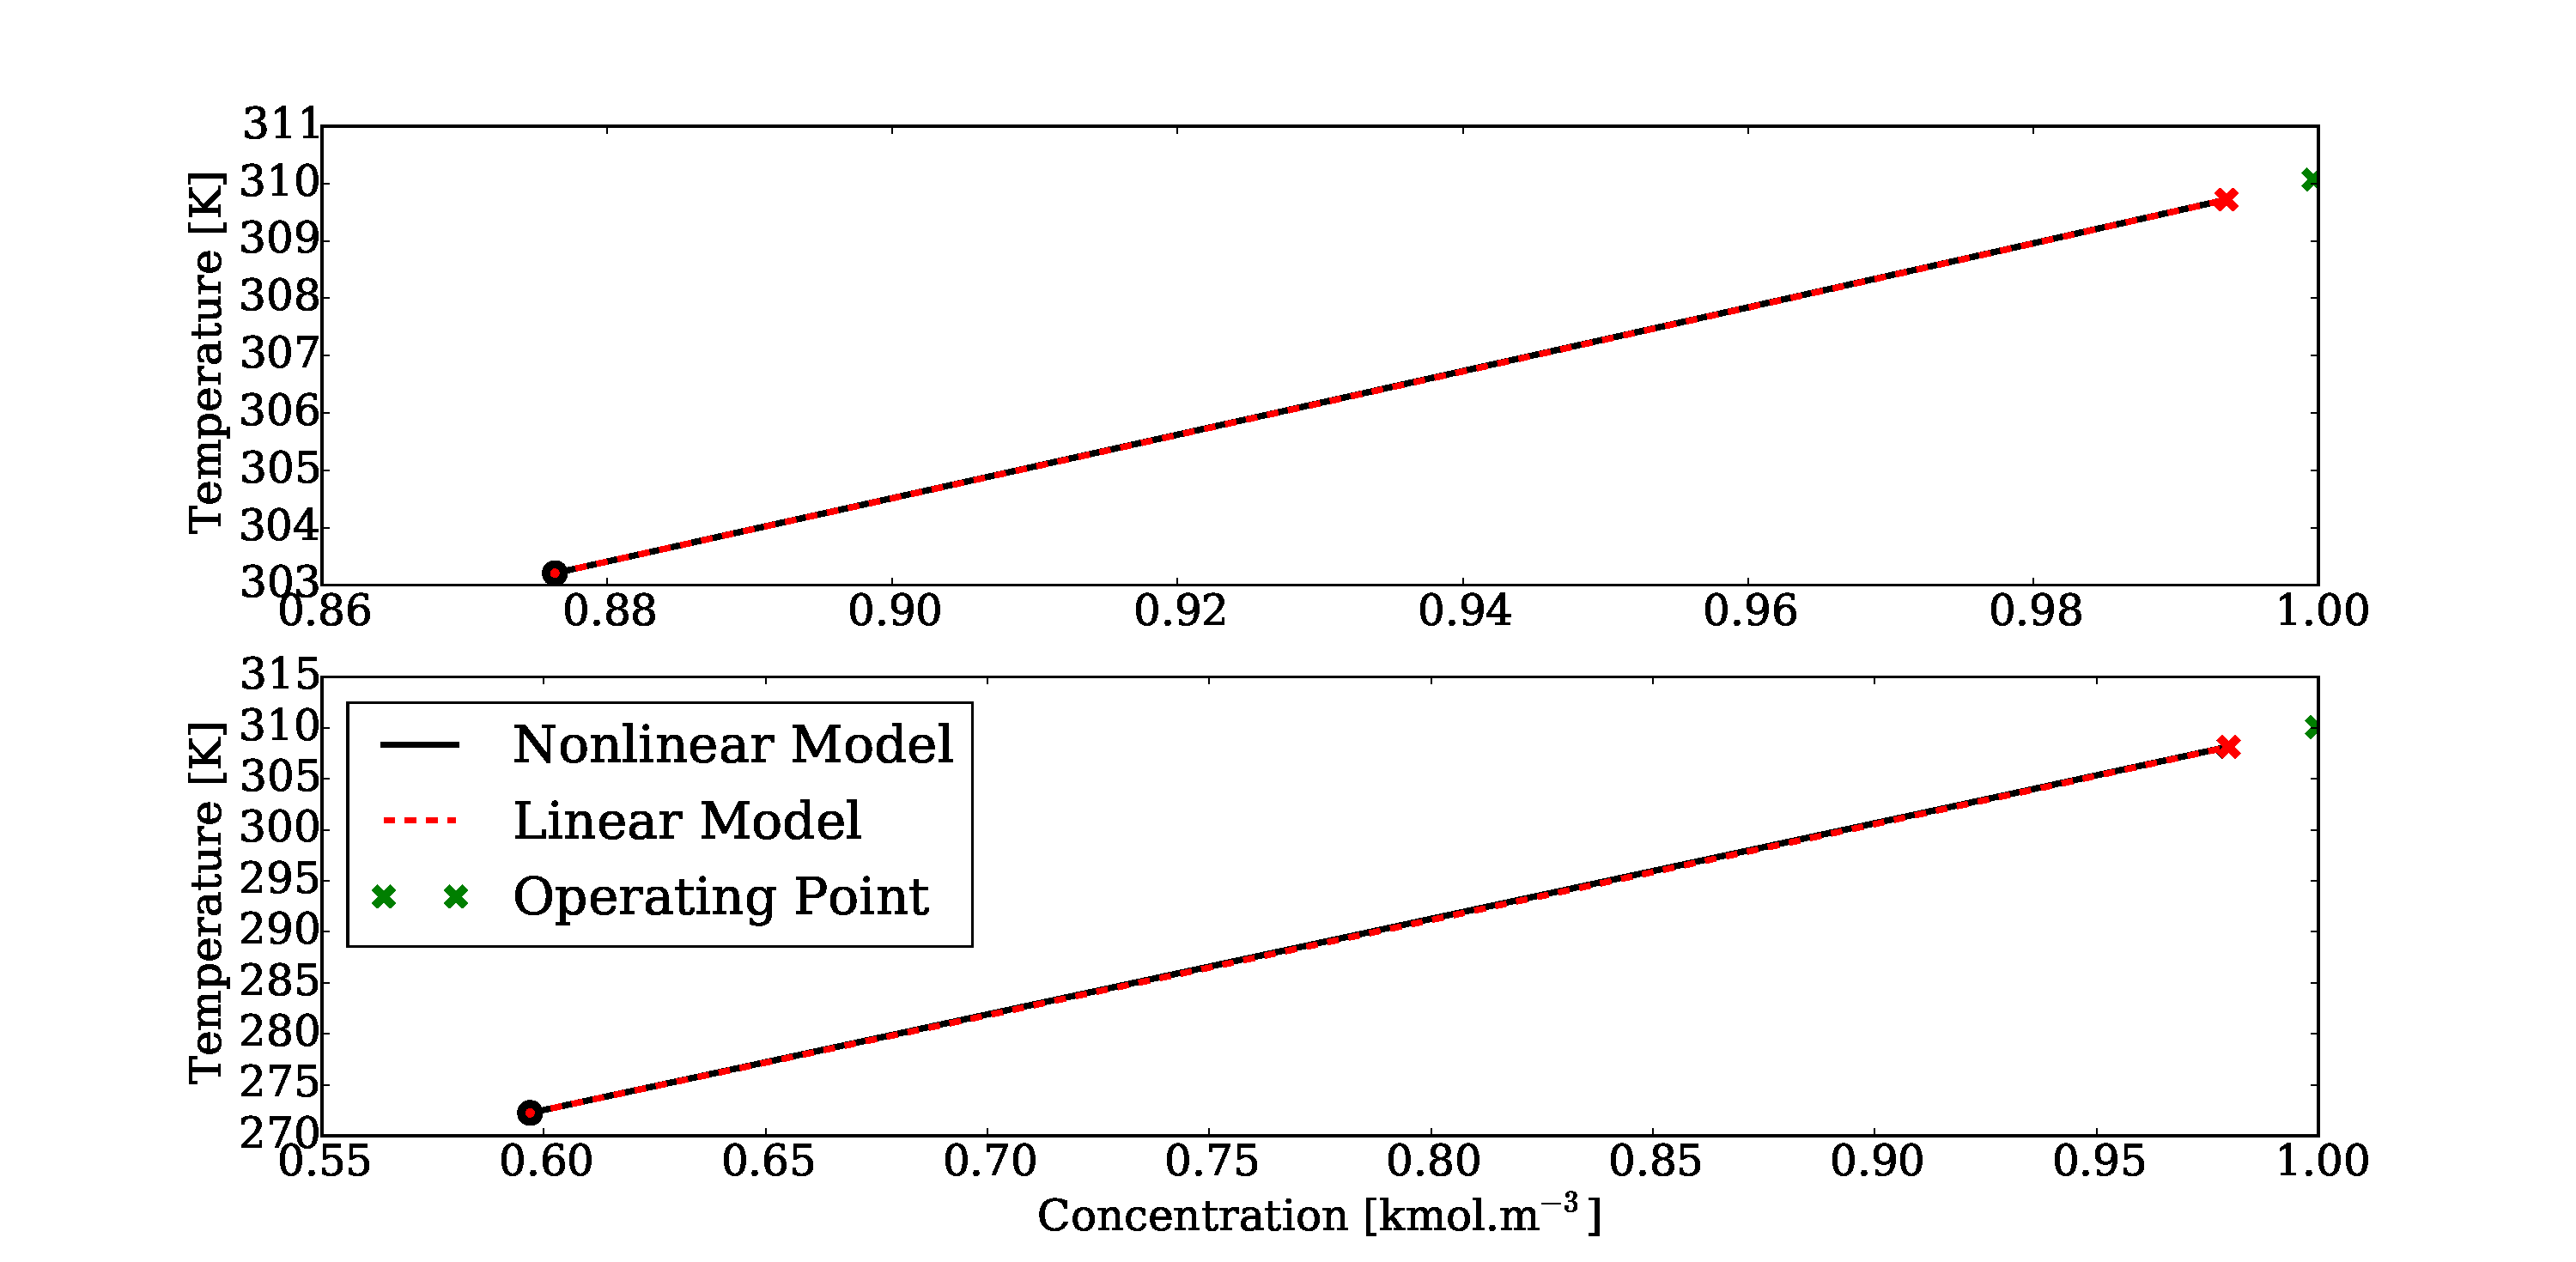
\includegraphics[width=\textwidth]{cstr_lin_3.pdf}
\caption{State space response of the CSTR under nominal operating conditions linearised around $(C_A^3,T_R^3)$ with different initial conditions. The dot indicates where the simulation started and the cross where it finished.}
\label{fig_cstr_lin_3}
\end{figure}
Like Figure \ref{fig_cstr_lin_1}, the linear model is quite accurate. The slow dynamics and stability of the operating point cause this desirable behaviour.

Based on the general linearisation formula in (\ref{eq_lin}) there is no reason why one cannot linearise about an arbitrary point in the state space. It stands to reason that the more linear models at different linearisation points one has, the better one will be able to model the reactor. For example, suppose one has 3 linear models. Each model will be more accurate in different regions of the state space. By selecting a model to use based on some metric (taking into account the current location in the state space) it is reasonable to suppose that one will be able to model the system more accurately than if only one linear model was available. In Part \ref{part_three} we take this idea further.

However, in Part \ref{part_two} we restrict our attention to systems where one linear model is sufficient for our purposes.  

